
\begin{widetext}
\begin{appendices} 
%\subsection{Definition and implications.}



%\section{Appendix A: Tables}
\label{appendix:tables}
Here we provide a brief map of our Appendices. In Appendix A, we provide numerical evidence for our main result, by plotting $\max_{\mathcal{NS}}\{p(S_2)\},\max_{{Q}}\{p(S_2)\}$  against observed values of an assorted bunch of tripartite non-locality measures. \textbf{Appendix B} contains the proof for \textbf{Property \ref{trivially_complementary_recurrence}.}  and \textbf{Property \ref{fixing_one_fixes_another}.}. \textbf{Appendix C}, contains the proof for \textbf{Theorem \ref{thm_1}.}. \textbf{Appendix D}, contains derivation of complementary relations between the winning probability of a $S_2$ game vs. single party marginals and of a $S_n$ game vs. single party marginals and $n-k$ party marginals.  
\textbf{Appendix E}, contains the proof of \textbf{Theorem \ref{thm_2}}.

 




\section{Other tripartite measures of non-locality vs. CHSH}
In this section, we provide numerical evidence for complementarity between tripartite genuine non-locality and bipartite non-locality using a selected bunch of tripartite measures and $p(S_2)$ as the bipartite measure of non-locality. Let us suppose, that a tripartite non-locality measure, $\mathcal{C}_3$ has an observed value $c$. Now, given this fact, we wish to find $\max_{\mathcal{NS}}p(S_2)$ and approximate $\max_{Q}p(S_2)$. Now, notice that the no-signaling constraints are linear on the conditional probabilities, hence, we solve the linear program of the form,

	
\begin{equation*}
\begin{aligned}
& {\text{maximize}}
& & p(S_2) \\
& \text{subject to}
& & \mathcal{C}_3=c, \\
&&& p(u_1,u_2,u_3|x_1,x_2,x_3)\in {\mathcal{NS}}.
\end{aligned}
\end{equation*}
Furthermore, we approximate using $Q_2$, a convex set of correlations, which approximates the quantum correlations. Its testing condition is a SDP program in the NPA hierarchy, 
	
\begin{equation*}
\begin{aligned}
& {\text{maximize}}
& & p(S_2) \\
& \text{subject to}
& & \mathcal{C}_3=c, \\
&&& p(u_1,u_2,u_3|x_1,x_2,x_3)\in {Q}_2.
\end{aligned}
\end{equation*}
We use two variations of Svetlichny's non-local game, $M_3,N_3$ \cite{barrett2005nonlocal,pironio2011extremal}. These differ from each-other and from $S_3$ in the way the inputs, $x_1,x_2,x_3$, are included the boolean condition for success. In both cases, complementarity relations are witnessed [see FIG. \ref{MG1},\ref{MG2}]. Next up, we use the Mermin's tripartite expression, $MF_3$. It is a Bell-type (CHSH like) expression, with 
local-real bound, $\max_{LV}\{MF_3\}=2$
equal no-signaling and quantum upper bounds, $\max_{\mathcal{NS}}\{MF_3\}=\max_Q\{MF_3\}=$. As discussed earlier, the violation of Mermin's inequality does not imply genuine multipartite non-locality, but just non-locality. As a result the characteristic complementarity is witnessed in the case of much tighter quantum constraints, \textit{no} complementarity is witnessed at all in the case of no-signaling constraints [see FIG. \ref{MF}]. \\
The correlations which can not be represented as in the form given in (\ref{SL}), are referred to as genuinely tripartite $SV_2$ non-local. While prescribing, (\ref{SL}), Svetlichny tacitly assumed that the measurements can 
 be regarded as simultaneous or the probabilities $p_{{\lambda}_1}(u_1,u_2|x_1x_2 ),p_{\lambda_2}(x_2 x_3|X_2X_3 ),p_{\lambda_3}(u_1,u_3|x_1,x_3 )$ are independent
of the timing of the measurements. This assumption goes well in the case, when the hidden variables are no signaling, otherwise, one might be faced with causality paradoxes. The polytope obtained using no-signaling hidden variables is referred to as $\mathcal{NS}_2$. An alternative solution to the causality puzzle is provided introducing the concept of time ordering in  
(\ref{SL}). The corresponding polytope obtained in this case is called $T_2$. It should be emphasized that $\mathcal{NS}_2 \subset T_2 \subset SV_2$ where the inclusion is strict. We compare $p(S_2)$ with the probabilistic expression, $I_3$. The violation of the corresponding inequality, implies that the correlations are $\mathcal{NS}_2$ and $T_2$ non-local.
Thus, $I_3\le0$ is a weaker (less stricter) inequality compared to the Svetlichny's inequality \cite{bancal2011definition}. Here, the complementarity is witnessed all the way from $I_3>0$ under both no-signaling and quantum constraints [see FIG. \ref{I}]. \\
Finally, we use the guess your neighbor's input game ($GYNI_n$) \cite{acin2016guess,pironio2011extremal}. This game consists of $n$ players, arranged on a ring, wherein each player receives a binary input $x_i$ for $i\in \{1,\ldots n\}$. The aim of the game is, to obtain a situation, wherein each player outputs a bit $u_i$ equal to the input bit of it's right neighbor, $u_i=x_{i-1}$. In case of $3$ players, the game is denoted as, $GYNI_{3}$. Here again, one can clearly visualize the complementarity relations [see FIG. \ref{GYNI}]. The expressions for these measures, their respective quantum and no-signaling bounds are presented in the Table \ref{bounds}. The plots for complementarity relations can be found in FIG. \ref{myTableSucks}. 
\begin{table}[!htb]
\centering
\begin{tabular} {|c|c|c|c|c|} 
\hline
%\diag{.1em}{3.48cm}{}{}
%{$p_{win}^{S_{n-1}}$}{$u_n,x_n$}
Tripartite Measure  \; &Expression \; & Quantum bound \;& No-signaling bound\; \\ \hline
$M_3$ & $u_1\oplus u_2\oplus u_3= x_1x_2x_3$ & $\frac{7}{8}$ & 1\\[5pt] \hline
$N_3$ & $u_1\oplus u_2\oplus u_3= x_1x_2 \oplus x_2x_3$&$\approx 0.7818$ & 1\\[5pt] \hline
$MF_3$ & \shortstack{~ $\langle x_1=1,x_2=0,x_3=0\rangle +\langle x_1=0,x_2=1,x_3=0\rangle$ \\ $+\langle x_1=0,x_2=0,x_3=1\rangle -\langle x_1=0,x_2=1,x_3=1\rangle$}& 4  & 4\\[5pt] \hline
$I_3$& \shortstack{~$-2p_{A_1A_2}(u_1=0,u_2=0|x_1=1,x_2=1)$ \\$-2p_{A_2A_3}(u_2=0,u_3=0|x_2=1,x_3=1)$ \\$-2p_{A_3A_1}(u_3=0,u_1=0|x_3=1,x_1=1)$\\$-p(u_1=0,u_2=0,u_3=0|x_1=0,x_2=0,x_3=1)$\\$-p(u_1=0,u_2=0,u_3=0|x_1=0,x_2=1,x_3=0)$\\$-p(u_1=0,u_2=0,u_3=0|x_1=1,x_2=0,x_3=0)$\\$+2p(u_1=0,u_2=0,u_3=0|x_1=0,x_2=1,x_3=1)$\\$+2p(u_1=0,u_2=0,u_3=0|x_1=1,x_2=0,x_3=1)$\\$+2p(u_1=0,u_2=0,u_3=0|x_1=1,x_2=1,x_3=0)$\\$+2p(u_1=0,u_2=0,u_3=0|x_1=1,x_2=1,x_3=1)$}& 0.14 & 0.5\\[5pt] \hline
$p(GYNI_3)$ & \shortstack{~ $p(u_1=0,u_2=0,u_3=0|x_1=0,x_2=0,x_3=0)$\\$+p(u_1=1,u_2=1,u_3=0|x_1=0,x_2=1,x_3=1)$\\$+p(u_1=0,u_2=1,u_3=1|x_1=1,x_2=0,x_3=1)$\\$+p(u_1=1,u_2=0,u_3=1|x_1=1,x_2=1,x_3=0)$}& 0.25 & $\frac{1}{3}$\\[5pt] \hline
\end{tabular}
\caption{Expressions for tripartite measures of non-locality, and their corresponding quantum and no-signaling upper bounds.} 
\label{Sncase2}
\label{bounds}
\end{table}

\begin{figure*}
\subfloat[\label{MG1} The observed winning probability in the $M_3$ game, $p(M_3)$.]{%
  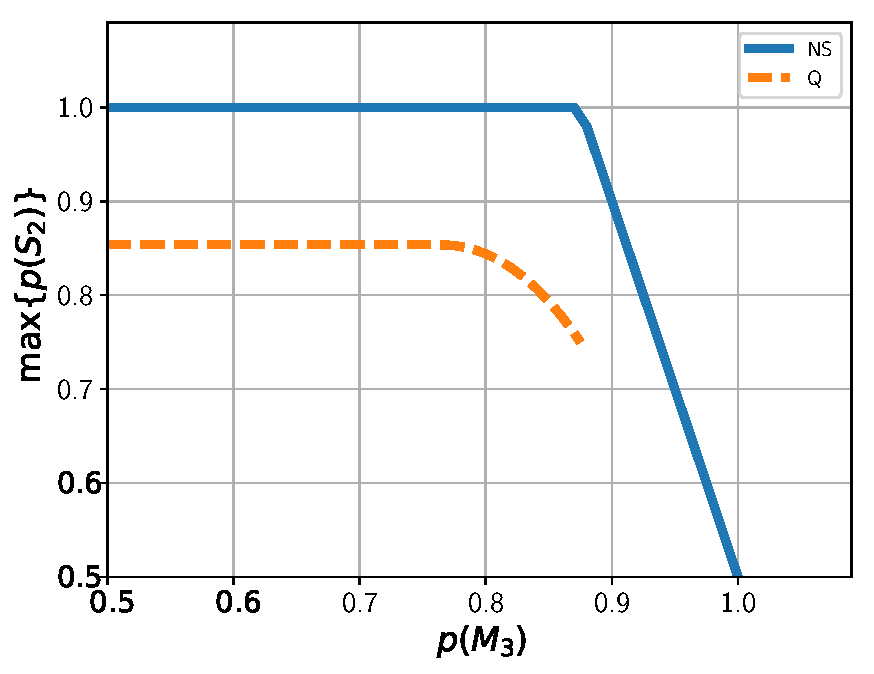
\includegraphics[scale=0.6]{images/chsh_vs_mg1.pdf}%
} \hfill
\subfloat[\label{MG2} The observed winning probability in the $N_3$ game, $p(N_3)$.]{%
  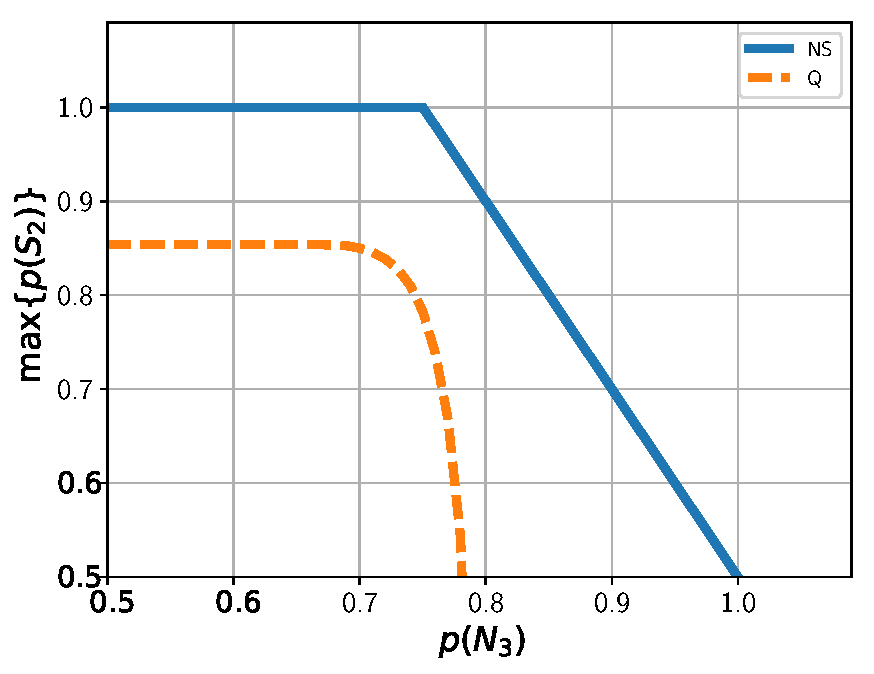
\includegraphics[scale=0.6]{images/chsh_vs_mg2.pdf}%
} \hfill
\subfloat[\label{MF} The observed value of Mermin's facet expression, $MF_3$.]{%
  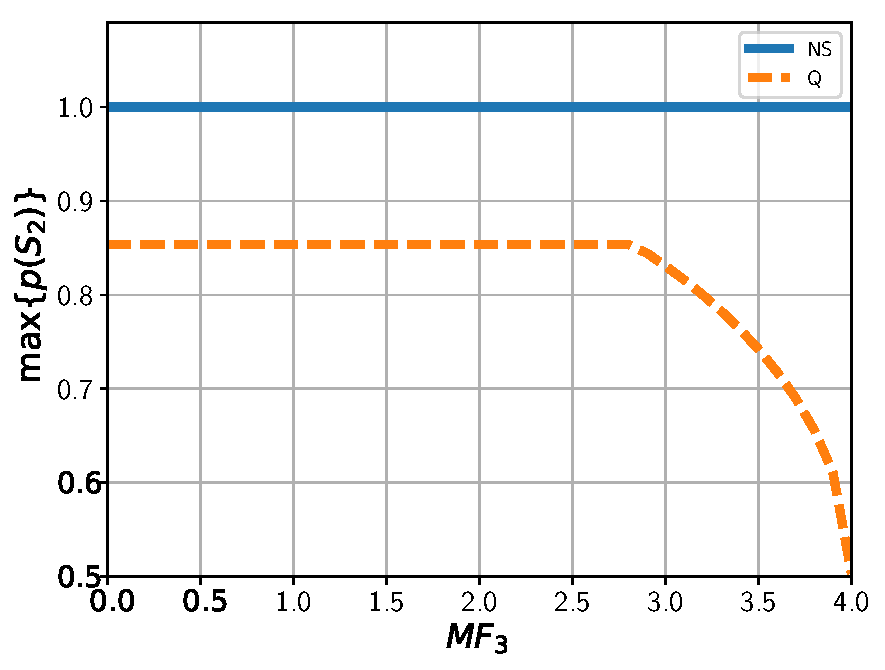
\includegraphics[scale=0.6]{images/chsh_vs_mf.pdf}%
} \hfill
\subfloat[\label{I} The observed value of $I_3$.]{%
  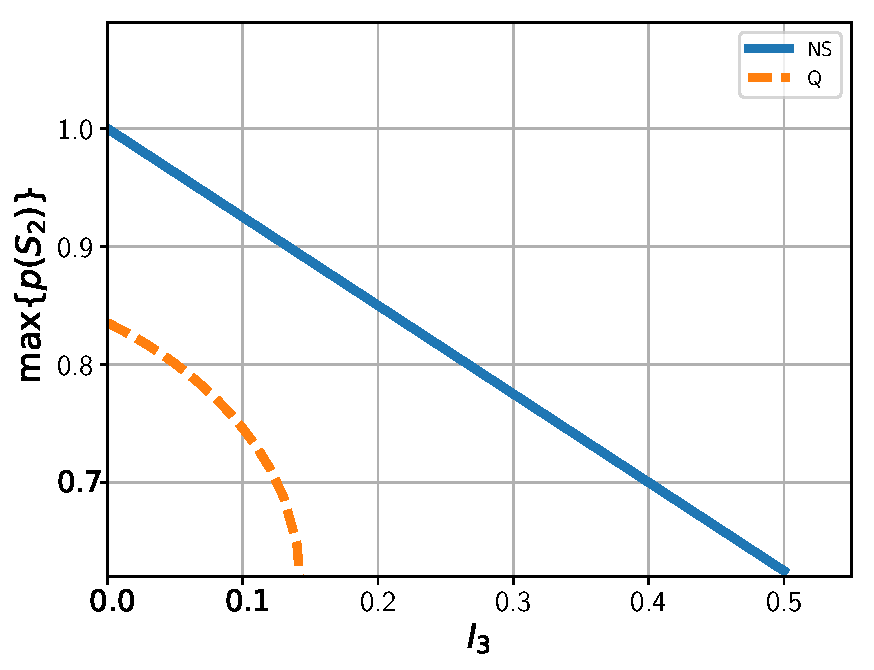
\includegraphics[scale=0.6]{images/chsh_vs_I.pdf}%
} \hfill
\subfloat[\label{GYNI} The observed winning probability in the GYNI game, $p(GYNI_3)$.]{%
  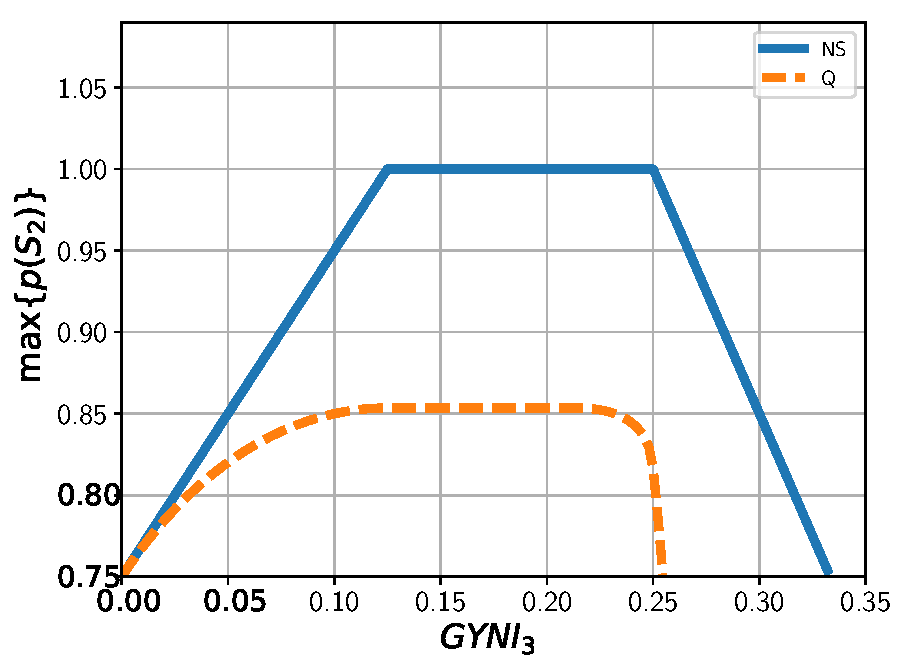
\includegraphics[scale=0.6]{images/chsh_vs_gyni.pdf}%
} \hfill
\caption{Plot of maximum achievable winning probability in a $S_2$ game, $\max \{p(S_2)\}$ against some tripartite measures of non-locality. For maximization over no-signaling probability distributions, the solid blue line, and for quantum probabilities, the dashed orange curve.
}
\label{myTableSucks}
\end{figure*}

 
\section{Decomposition of $S_n$-games}
\label{svet_prop}
\noindent A $n$-party Svetlichny's non-local game, $S_n^i$, reduces to four $n-1$-party Svetlichny's non-local games, given the fixed assignment of the input and output bits of the $n$th party, denoted by $S_{n-1}^j\equiv S_n^i|(u_n=u_n',x_n=x_n')$, for  $u_n',x_n' \in \{0,1\}$. Similarly, a $S_n^j$ game reduces to four $k$-party Svetlichny's non-local games, given the fixed assignment of the input and output bits of $n-k$ parties, denoted by $S_{k}^j\equiv S_n^i|(u_{k+1}=u_{k+1}',\ldots u_n=u_n',x_{k+1}=x_{k+1}',\ldots x_n=x_n')$ where $u_i',x_i'\in \{0,1\}$ for $k < i \le n$. If $S_n^i$ game is of the form (\ref{svetlichny_recurssive}), then the $S_{k}^j$ game, thus obtained, is given by,
%\begin{widetext}
\begin{eqnarray}
\label{svetlichny_in_any_lower_form}
&&(\bigoplus_{1\le i \le k}u_i) \oplus (\bigoplus_{k < i \le n}u_i{'}) \oplus c_0 ={}\nonumber\\&&
(\bigoplus_{1\le i<j \le k}x_i x_j) \oplus
 (\bigoplus_{1 \le i \le k} (\bigoplus_{k<j\le n}x_{j}{'} \oplus c_i ) \ x_i) \oplus
 (\bigoplus_{k<i \le n}c_ix_i{'}) \; . {}\nonumber\\&&  
\end{eqnarray} 
Using the definitions of $\mathcal{A}_{n-k},\mathcal{B}_{n-k}$, we can rewrite the above as,
%\begin{widetext}
\begin{eqnarray}
\label{svetlichny_k_00}
&& S_k^1 \equiv S_{n}^j|( \mathcal{A}_{n-k}=0,\mathcal{B}_{n-k}=0) \equiv  {}\nonumber\\&&
\bigoplus_{1 \le i\le k} u_i \oplus c_0 = 
(\bigoplus_{1 \le i<j \le k} x_i x_j) \oplus (\bigoplus_{1 \le i\le k}c_i x_i) {} \; ,\nonumber\\&& 
{S_k^1}' \equiv S_{n}^j|(\mathcal{A}_{n-k}=1,\mathcal{B}_{n-k}=0) \equiv {}\nonumber\\&&  
\bigoplus_{1 \le i\le k} u_i \oplus c_0 \oplus 1 = 
(\bigoplus_{1 \le i<j \le k} x_i x_j) \oplus (\bigoplus_{1 \le i\le k}c_i x_i) {} \ ,\nonumber\\&&  
S_k^2 \equiv S_{n}^j|(\mathcal{A}_{n-k}=0,\mathcal{B}_{n-k}=1) \equiv {}\nonumber\\&&  
\bigoplus_{1\le i\le k} u_i \oplus c_0 =
 (\bigoplus_{1 \le i<j \le k} x_i x_j) \oplus (\bigoplus_{1 \le i\le k}(1\oplus c_i) x_i) {} \ ,\nonumber\\&& 
{S_k^2}'\equiv S_{n}^j|(\mathcal{A}_{n-k}=1,\mathcal{B}_{n-k}=1) \equiv {}\nonumber\\&&
\bigoplus_{1 \le i \le k} u_i \oplus c_0 \oplus 1 = 
(\bigoplus_{1 \le i,j \le k} x_i x_j) \oplus  (\bigoplus_{1 \le i \le k}(1\oplus c_i) x_i)  {} \; .\nonumber\\&& 
\end{eqnarray}
The equation (\ref{svetlichny_k_00}) reveals that the game $S_n^j$ game decomposes into one of the four games: ${S_k^1},{S_k^1}',{S_k^2},{S_k^2}'$ depending on the value of the boolean expressions $\mathcal{A}_{n-k}$ and $\mathcal{B}_{n-k}$. Moreover, the following relation holds between the $S_k^1$ game and $S_k^2$ game,
\begin{eqnarray}
\label{rel_for_fiu_one_fiu_another}
&&S_k^1  \equiv
S_k^2 \oplus \bigoplus_{1 \le i \le k}x_i \; .
\end{eqnarray}
Also from \textbf{Property \ref{trivially_complementary_recurrence}.}, it follows that the same relation holds between ${S_k^1}'$ game and ${S_k^2}'$ game, respectively. \\   

%\end{widetext}






\section{ Proof of Theorem 1}
We shall now give the proof for \textbf{Theorem \ref{thm_1}.} using induction. First, we show that the relations hold for $n=1$. 
\subsection*{$S_1$ vs. $S_1$}
Consider the four single party games $S_1^1\equiv u_1=0$, ${S_1^1}'\equiv u_1=1$, ${S_1^2}\equiv u_1=x_1$ and ${S_1^2}'\equiv x_1\oplus 1$  obtained from (\ref{svetlichny_recurssive}) for $n=1$. We want to find, $\max\{p(S_1^2)\}$ for a given value of $p({S_1^1}) \in [\frac{1}{2},1] $. Using the fact that, $p({S_1^1})=\frac{p(u_1=0|x_1=0)+p(u_1=0|x_1=1)}{2}$ and $p({S_1^2})=\frac{p(u_1=0|x_1=0)+p(u_1=1|x_1=1)}{2}$, we get $p({S_1^2}) + p({S_1^1}) = \frac{1+2p(u_1=0|x_1=0)}{2}$. Now, $\max\{p(u_1=0|x_1=0)\}=1$, which leads one to $\max\{p(S_1^2)\}=\frac{3}{2}-p({S_1^1})$. Notice, for $p({S_1^1})\in [0,\frac{1}{2})$, $p(u_1=0|x_1=0)$ cannot be $1$. So we shall consider, $p({S_1^2}) - p({S_1^1}) = \frac{1-2p(u_1=0|x_1=1)}{2}$. Now, $\min\{p(u_1=0|x_1=1)\}=0$, which yields, $\max\{p(S_1^2)\}=\frac{1}{2}+p({S_1^1})=\frac{3}{2}-p({S_1^1}')$.  
So in general, we have for a given value $p(S_1^i)$, $\max\{p(S_1^j)\}$ is given by,
\begin{eqnarray}
\label{marginal_game}
    \max_{\mathcal{NS}} \{ p({S_1^j}) \} =
    \begin{cases}
      p({S_1^i}), & \text{if}\ S_1^j \equiv S_1^i \\
      1 - p({S_1^i}), & \text{if}\ S_1^j \equiv {S_1^i}{'}   \\
      p({S_1^i})+\frac{1}{2}, &  \text{if} \ S_1^j \not \equiv \{{S_1^i},{S_1^i}{'}\},  p({S_1^i})\le \frac{1}{2} \\
      
      -p({S_1^i}) +\frac{3}{2}, & \text{if} \ S_1^j \not \equiv \{{S_1^i},{S_1^i}{'}\},  p({S_1^i}) \ge \frac{1}{2} \ . \\
     
    \end{cases} 
\end{eqnarray}
\noindent
Notice that here we \textit{did not} use any constrains on the conditional probability distribution $p(u_1|x_1)$, hence, this stands true for classical, quantum and no-signaling restrictions.\\
\subsection*{$S_n$ vs. $S_n$}
Now for the proof for any $n$, as the next step of induction, we assume that the complementary relation presented in \textbf{Theorem 1.}, holds for $S_{n-1}$ games, and consequently prove 
the same for $S_n$ games. Let us consider two $S_n$ games, $S_n^i$ and $S_n^j$ which are neither equivalent nor trivially 
complementary to each other. In addition, we consider only the case when $ p(S_n^i)\geq \frac{1}{2}$. The winning probability of the $S_n^i$ game can be expressed as,
\begin{eqnarray}
\label{S_n__vs__S_n__1}
%\begin{eqnaraay}
&&p({S_n^i}) ={}\nonumber\\&& \frac{1}{2} \bigg( p(u_n=0|x_n=0)(p({S_{n-1}^1}|u_n=0,x_n=0){}\nonumber\\&&+p(u_n=1|x_n=0)(p({{S_{n-1}^1}{'}}|u_n=1,x_n=0){}\nonumber\\&&
+p(u_n=0|x_n=1)(p({S_{n-1}^2}|u_n=0,x_n=1){}\nonumber\\&&+p(u_n=1|x_n=1)(p({{S_{n-1}^2}{'}}|u_n=1,x_n=1) \bigg) \; ,
\nonumber\\&&
%\end{split} 
\end{eqnarray}
where ${S_{n-1}^1} \equiv S_{n}^i||(u_n=0,x_n=0)$,
${{S_{n-1}^1}{'}} \equiv S_{n}^i|(u_n=1,x_n=0)$,${S_{n-1}^2} \equiv S_{n}^i||(u_n=0,x_n=1)$,
${{S_{n-1}^2}{'}} \equiv S_{n}^i|(u_n=1,x_n=1)$.  Similarly, the winning probability of the $S_n^i$ game can be expressed as, 
\begin{eqnarray}
\label{S_n__vs__S_n__2}
%\begin{eqnaraay}
&&p({S_n^j}) ={}\nonumber\\&& \frac{1}{2} \bigg( p(u_n=0|x_n=0)(p({S_{n-1}^3}|u_n=0,x_n=0){}\nonumber\\&&+p(u_n=1|x_n=0)(p({S_{n-1}^3}{'}|u_n=1,x_n=0){}\nonumber\\&&
+p(u_n=0|x_n=1)(p({S_{n-1}^4}|u_n=0,x_n=1){}\nonumber\\&&+p(u_n=1|x_n=1)(p({{S_{n-1}^4}{'}}|u_n=1,x_n=1) \bigg) \; . \nonumber\\&& 
%\end{split}
\end{eqnarray}
Now, one can write no-signaling condition as,
\begin{equation}
\begin{split}
p(u_n=0|x_n=0)p(u_1,\ldots u_{n-1}|x_1,\ldots x_n)_{u_n=0,x_n=0}+p(u_n=1|x_n=0)p(u_1,\ldots u_{n-1}|x_1,\ldots x_n)_{u_n=1,x_n=0}= \\
p(u_n=0|x_n=1)p(u_1,\ldots u_{n-1}|x_1,\ldots x_{n-1})_{u_n=1,x_n=1}+p(u_n=1|x_n=1)p(u_1,\ldots u_{n-1}|x_1,\ldots x_{n-1})_{u_n=1,x_n=1}.
\end{split}
\end{equation}
Notice that the winning probability of any $S_{n-1}$ game is sum over specific probabilities of the form $p(u_1,u_2,\ldots,u_{n-1}|x_1,x_2,\ldots,x_{n-1})$, therefore we can state the no-signaling condition for any particular $S_{n-1}^j$ game,
\begin{equation}
\label{no_signaling_conx_indp_of_input}
\begin{split}
&~~p(u_n=0|x_n=0)(p(S_{n-1}^j|u_n=0,x_n=0))  \\ &+p(u_n=1|x_n=0)(p(S_{n-1}^j|u_n=1,x_n=0))  \\
&= p(u_n=0|x_n=1)(p(S_{n-1}^j|u_n=0,x_n=1))  \\ &+p(u_n=1|x_n=1)(p(S_{n-1}^j|u_n=1,x_n=1))\; .
\end{split}
\end{equation}
% In addition to Eq. \ref{S_n__no_signaling}, no-signaling condition necessitates that values of $p_{win}^{s_{n-1}}$ for $S_{n-1}$ games are in accordance with Eq. \ref{marginal_game} for any fixed values of $u_n$ and $x_n$. \\
\noindent From \textbf{Property \ref{trivially_complementary_recurrence}.} and \textbf{Property \ref{fixing_one_fixes_another}.} we have the following two representative cases:
\begin{enumerate}
\item $ S_{n-1}^1,S_{n-1}^2  \not \in \{S_{n-1}^3, {S_{n-1}^3}{'},S_{n-1}^4, {S_n^4}{'}\}$: Following from the observation in ($S_n$ vs. marginals), we shall fix the marginals of the $n$th party to be $\frac{1}{2}$, i.e., $p(u_n|x_n)=\frac{1}{2}$. Now, for $p(S_n^i) \ge \frac{1}{2}$ let us suppose that, $p(S_n^i)=\frac{1}{2}+\delta$ for some $\delta\in [0,\frac{1}{2}]$. Furthermore, we assume w.l.o.g. that, $p(S_{n-1}^1|u_n=0,x_n=0)=\frac{1}{2}+\delta_1$, $(p({S_{n-1}^1}{'}|u_n=1,x_n=0)=\frac{1}{2}+\delta_2$,  $p(S_{n-1}^2|u_n=0,x_n=1)=\frac{1}{2}+\delta_3$ and  $p({S_{n-1}^2}{'}|u_n=1,x_n=1)=\frac{1}{2}+\delta_4$ where $\delta_i \in [-\frac{1}{2},\frac{1}{2}]$ for $i \in \{0,1,2,3\}$. Therefore, $\delta=\frac{1}{4}\sum_i\delta_i$.
Now, from the assumption of involved in induction, that the $S_{n-1}$ follow the relation presented in \textbf{Theorem \ref{thm_1}.}, we obtain $\max_{\mathcal{NS}} \{p(S_n^j)\}=1-\frac{1}{4}\sum_i\delta_i=1-\delta=\frac{3}{2}-p({S_n^i})$. For the purpose of illustration, we provide the optimal assignment in the form of the Table \ref{Sncase1}, with $\delta_1=\delta_2=\delta_3=\delta_4=\delta$. Notice, that sum of values in first two columns is equal to that of the last two columns, thus condition in (\ref{no_signaling_conx_indp_of_input}) is satisfied. Also, all $S_{n-1}$ games satisfy the complementary relations given in \textbf{Theorem \ref{thm_1}.}.
\begin{table}[!htb]
\centering
\begin{tabular} {|l|l|l|l|l|} 
\hline
%\diag{.1em}{3.48cm}{}{}
%{$p_{win}^{S_{n-1}}$}{$u_n,x_n$}
&$u_n=0,x_n=0$&$u_n=1,x_n=0$&$u_n=0,x_n=1$&$u_n=1,x_n=1$\tabularnewline \hline
$p({S_{n-1}^1}|u_n,x_n)$& $\frac{1}{2}+\delta$ & $\frac{1}{2}-\delta$ & $1-\delta$&$\delta$\tabularnewline \hline
$p({S_{n-1}^1}{'}|u_n,x_n)$& $\frac{1}{2}-\delta$ & $\frac{1}{2}+\delta$ & $\delta$ &$1-\delta$\tabularnewline \hline
$p({S_{n-1}^2}|u_n,x_n)$&$1-\delta$ & $\delta$ & $\frac{1}{2}+\delta$&$\frac{1}{2}-\delta$\tabularnewline \hline
$p({S_{n-1}^2}{'}|u_n,x_n)$& $\delta$ & $1-\delta$ & $\frac{1}{2}-\delta$ &$\frac{1}{2}+\delta$\tabularnewline \hline
\end{tabular}
\caption{\label{Sncase1} Optimal assignment for case 1. }
\end{table}
\item $S_{n-1}^1 \equiv S_{n-1}^3$   and $S_{n-1}^2  \equiv {S_{n-1}^4}{'}$: Here, proceeding with notations and assumptions of the previous case, we find that it is possible to fix $(p({S_{n-1}^1}|u_n=0,x_n=0)=(p({{S_{n-1}^1}{'}}|u_n=1,x_n=0)=1$. Such that $\delta=\frac{1+\delta_3+\delta_4}{4}$. Again, from the assumption that $S_{n-1}$ games follow the relation presented in \textbf{Theorem \ref{thm_1}.}, we obtain $\max_{\mathcal{NS}}\{p(S_n^j)\}=1-\frac{(1+\delta_3+\delta_4)}{4}=1-\delta=\frac{3}{2}-p(S_n^i)$. Yet again, for the purpose of illustration, we provide the optimal assignment in the form of the Table \ref{Sncase1}, with $\delta_1=\delta_2=\delta_3=\delta_4=\delta$. Notice, that sum of values in first two columns is equal to that of the last two columns, thus condition in (\ref{no_signaling_conx_indp_of_input}) is satisfied. Also, all $S_{n-1}$ games satisfy the complementary relations given in \textbf{Theorem \ref{thm_1}.}.
\begin{table}[!htb]
\centering
\begin{tabular} {|l|l|l|l|l|} 
\hline
%\diag{.1em}{3.48cm}{}{}
%{$p_{win}^{S_{n-1}}$}{$u_n,x_n$}
&$u_n{'}=0,x_n{'}=0$&$u_n{'}=1,x_n{'}=0$&$u_n{'}=0,x_n{'}=1$&$u_n{'}=1,x_n{'}=1$\\ \hline

$p({S_{n-1}^1}'|u_n,x_n)$& $1$ & $0$ & $\frac{1}{2}$&$\frac{1}{2}$\\ \hline

$p({S_{n-1}^1}'|u_n,x_n)$& $0$ & $1$ & $\frac{1}{2}$ &$\frac{1}{2}$\\ \hline

$p({S_{n-1}^2}|u_n,x_n)$&$\frac{1}{2}$ & $\frac{1}{2}$ & $2\delta$&$1-2\delta$\\ \hline

$p({S_{n-1}^2}'|u_n,x_n)$& $\frac{1}{2}$ & $\frac{1}{2}$ & $1-2\delta$ &$2\delta$\\ \hline
\end{tabular}

\caption{Optimal assignment for case 2.} 
\label{Sncase2}
\end{table}
\end{enumerate} 
All other cases, can be handled using the above to cases.
\section{Complementarity with Marginals}
\subsection*{ $S_2$ {vs. marginals} }
\noindent
Consider a bipartite Svetlichny's non-local game, $S_2 \equiv u_1 \oplus u_2 =x_1x_2$. Its winning probability can be rewritten as,
%\begin{widetext}
\begin{eqnarray}
\label{Chsh_vs_marginal_pwin_breakdown}
%\begin{eqnaraay}
p(S_2) &&= \frac{1}{4} \bigg( p(u_2=0|x_2=0)(p(u_1=0|x_1=0)+p(u_1=0|x_1=1))_{u_2=0,x_2=0}
{}\nonumber\\&&+p(u_2=1|x_2=0)(p(u_1=1|x_1=0)+p(u_1=1|x_1=1))_{u_2=1,x_2=0}
{}\nonumber\\&&
+p(u_2=0|x_2=1)(p(u_1=0|x_1=0)+p(u_1=1|x_1=1))_{u_2=0,x_2=1}{}\nonumber\\&&+p(u_2=1|x_2=1)(p(u_1=1|x_1=0)+p(u_1=0|x_1=1))_{u_2=1,x_2=1} \bigg) {} \; ,
%\end{split} 
\end{eqnarray}
%\end{widetext}
%\begin{equation}
%p_{win}^{CHSH}=\frac{\sum_{X.Y=a\uplus b}p(a,b|X,Y)}{4}
%\end{equation}
%which may also is written in the form,
%\begin{equation}\label{CHSHtut}
%p^{CHSH}_{win}=\sum_{i,j}{\frac{p(b=i|Y=j)\sum_{X.j=a\oplus i}(a |X,b=i,Y=j)}{4}}
%\end{equation}
\noindent
where $()_{u_2=i,x_2=j}$ indicates the fact that all probabilities contained within the brackets are conditioned on $u_2=i,x_2=j$. Let $p(u_2=0|x_2=0)=\mathsf{p}$ and $p(u_2=0|x_2=1)=\mathsf{p}'$, 
then no-signaling condition
from $A_2$ to $A_1$ can be stated as,
%\begin{widetext}
\begin{eqnarray}
\label{chsh_vs_marginal_no_signaling_condition_1}
&&\mathsf{p}p(u_1=0|x_1=0)_{u_2=0,x_2=0}+(1-\mathsf{p})p(u_1=0|x_1=0)_{u_2=1,x_2=0}={}\nonumber\\&&
\mathsf{p}'p(u_1=0|x_1=0)_{u_2=0,x_2=1}+(1-\mathsf{p}')p(u_1=0|x_1=0)_{u_2=1,x_2=1} \; ,
\end{eqnarray}
\begin{eqnarray}
\label{chsh_vs_marginal_no_signaling_condition_2}
&&\mathsf{p}p(u_1=0|x_1=1)_{u_2=0,x_2=0}+(1-\mathsf{p})p(u_1=0|x_1=1)_{u_2=1,x_2=0}={}\nonumber\\&&
\mathsf{p}'p(u_1=0|x_1=1)_{u_2=0,x_2=1}+(1-\mathsf{p}')p(u_1=0|x_1=1)_{u_2=1,x_2=1} \; .
\end{eqnarray}
%\end{widetext}
Now, in-order to find $\max_{\mathcal{NS}} \{p({S_2})\}$, we fix
$p(u_1=0|x_1=0)_{u_2=0,x_2=0}=1$ ,$p(u_1=1|x_1=0)_{u_2=1,x_2=0}=1$,$p(u_1=0|x_1=0)_{u_2=0,x_2=1}=1$ and $p(u_1=1|x_2=0)_{u_2=1,x_2=1}=1$ and obtain $\mathsf{p}=\mathsf{p}{'}$ from (\ref{chsh_vs_marginal_no_signaling_condition_1}). Further fixing $p(u_1=0|x_1=1)_{u_2=0,x_2=0}=1$,  $p(u_1=1|x_1=1)_{u_2=1,x_2=0}=1$,  $p(u_1=1|x_1=1)_{u_2=0,x_2=1}=1$, we obtain $p(u_1=0|x_1=1)_{u_2=1,x_2=1}=\frac{\mathsf{p}}{1-\mathsf{p}}$ for $p\in [0,\frac{1}{2}] $ and  $p(u_1=0|x_2=1)_{u_2=1,x_2=1}=\frac{1-\mathsf{p}}{\mathsf{p}}$ for $\mathsf{p}\in [\frac{1}{2},1] $ from  (\ref{chsh_vs_marginal_no_signaling_condition_2}). This in-turn leads us to, 
\begin{equation}
\label{chsh_marginal_result}
    \max_{\mathcal{NS}} \{ p({S_2})\} =
    \begin{cases}
      \frac{3+2\mathsf{p}}{4}, & \text{if}\ \mathsf{p}\in[0,\frac{1}{2}]\\
      \frac{5-2\mathsf{p}}{4}, & \text{if}\ \mathsf{p}\in[\frac{1}{2},1] \; .\\
     \end{cases} 
\end{equation}

\subsection*{${S_n}$ {vs. marginals}}
\noindent
Now we prove that the complementary relation of the type given by ( \ref{chsh_marginal_result}), hold for $S_n$ games with $n \ge 3$. W.l.o.g., we consider, $S_n \equiv  \bigoplus_{1\le i \le n} u_i = \bigoplus_{1\le i<j \le n} x_i x_j$. We define $A=\bigoplus_{1\le i \le n-1}u_i$, $B=\bigoplus_{1\le i<j \le n-1}x_ix_j$ and $C=\bigoplus_{1\le i \le n-1}x_i$. Also let $p(u_n=0|x_n=0)=\mathsf{p}$ and $p(u_n=0|x_n=1)=\mathsf{p}{'}$. Then the winning probability of the $S_n$-game can be rewritten as,
\begin{eqnarray}
\label{S_n_vs_marginal_win_probability}
p({S_n^i}) &&= \frac{1}{2^n} \Bigg( p(u_n=0|x_n=0)(p(A=B))_{u_n=0,x_n=0}
{}\nonumber\\&&+p(u_n=1|x_n=0)(p(A=B\oplus1))_{u_n=1,x_n=0}{}\nonumber\\&&
+p(u_n=0|x_n=1)(p(A=B\oplus C))_{u_n=0,x_n=1}
{}\nonumber\\&&+p(u_n=1|x_n=1)(p(A=B\oplus C \oplus 1))_{u_n=1,x_n=1} \Bigg)  \; ,
\end{eqnarray}
where $()_{u_2=i,x_2=j}$ indicates the fact that all probabilities contained within the brackets are conditioned on $u_2=i,x_2=j$.To proceed further, we consider the following two cases:
\begin{enumerate}
\item First we consider an assignment of input bits, such that $C=0$. The no-signaling can be rewritten as,
\begin{eqnarray}
\label{S_n_vs_marginal_case_1}
\mathsf{p}(p(A=B))_{u_n=0,x_n=0}+(1-\mathsf{p})(p(A=B))_{u_n=1,x_n=0} \\=
\mathsf{p}{'}(p(A=B))_{u_n=0,x_n=1}+(1-\mathsf{p}{'})(p(A=B))_{u_n=1,x_n=1}
{}\nonumber \; .
\end{eqnarray}
To maximize $p({S_n})$ we keep $(p(A=B))_{u_n=0,x_n=0}=(p(A=B))_{u_n=0,x_n=1}=1$ and $(p(A=B))_{u_n=1,x_n=0}=(p(A=B))_{u_n=1,x_n=1}=0$ in (\ref{S_n_vs_marginal_case_1}), obtaining $\mathsf{p}=\mathsf{p}{'}$.
\\
\item Now, we consider an assignment of input bits, such that $C=1$. In this case, in-order to maximize $p({S_n})$, we keep 
$(p(A=B))_{u_n=0,x_n=0}=1$ and $(p(A=B))_{u_n=1,x_n=0}=(p(A=B))_{u_n=0,x_n=1}=0$ in (\ref{S_n_vs_marginal_case_1}), getting $(p(A=B))_{u_n=1,x_n=1}=\frac{\mathsf{p}}{1-\mathsf{p}}$ for $\mathsf{p} \le \frac{1}{2}$ (and $\frac{1-\mathsf{p}}{\mathsf{p}}$ for $\mathsf{p} \ge \frac{1}{2}$, obtained by replacing $\mathsf{p}$ by $1-\mathsf{p}$).
\end{enumerate}
As there are $2^{n-2}$ assignment of input bits possible, for $C=0$ and $C=1$, keeping the values of terms (\ref{S_n_vs_marginal_win_probability}) according to that described in above two cases, we get the same expression for $\max_{\mathcal{NS}}  \{p({S_n})\}$, as given in (\ref{chsh_marginal_result}).


\subsection*{${S_n}$ {vs. auxiliary games}}
We again consider the following $S_n$ game $S_n^i \equiv  \bigoplus_{1\le i \le n} u_i = \bigoplus_{1\le i<j \le n} x_i x_j$ ( it can be proved similarly for other $S_n$ games ).
We define $A=\bigoplus_{1\le i \le k}u_i$, $B=\bigoplus_{1\le i<j \le k}x_ix_j$ and $C=\bigoplus_{1\le i \le k}x_i$. Also fix $p(\mathcal{A}_{n-k}=0|\mathcal{B}_{n-k}=0)=p$ and $p(\mathcal{A}_{n-k}=0|\mathcal{B}_{n-k}=1)=p{'}$ ( where $A_n^k$ and $B_n^k$ are defined according to Eq. \ref{aux1} and \ref{aux2} ). Using Eq. \ref{general_win_probability2}

\begin{eqnarray}
\label{S_n_vs_marginal_win_probability2}
p_{win}^{S_n^i} &&= \frac{1}{2^{k+1}} \Bigg( p(\mathcal{A}_{n-k}=0|\mathcal{B}_{n-k}=0)\bigg(\sum_{x_1{'},\ldots ,x_{k}{'} \in \{0,1\}}p(A=B|x_1=x_1{'},\ldots x_{k}=x_{k}{'})\bigg)_{\mathcal{A}_{n-k}=0,\mathcal{B}_{n-k}=0}
{}\nonumber\\&&+p(\mathcal{A}_{n-k}=1|\mathcal{B}_{n-k}=0)\bigg(\sum_{x_1{'},\ldots x_{k}{'} \in \{0,1\}}p(A=B\oplus1|x_1=x_1{'},\ldots x_{k}=x_{k}{'})\bigg)_{\mathcal{A}_{n-k}=1,\mathcal{B}_{n-k}=0}{}\nonumber\\&&
+p(\mathcal{A}_{n-k}=0|\mathcal{B}_{n-k}=1)\bigg(\sum_{x_1{'},\ldots x_{k}{'} \in \{0,1\}}p(A=B\oplus C|x_1=x_1{'},\ldots x_{k}=x_{k}{'})\bigg)_{\mathcal{A}_{n-k}=0,\mathcal{B}_{n-k}=1}
{}\nonumber\\&&+p(\mathcal{A}_{n-k}=1|\mathcal{B}_{n-k}=1)\bigg(\sum_{x_1{'},\ldots x_{k}{'} \in \{0,1\}}p(A=B\oplus C \oplus 1|x_1=x_1{'},\ldots x_{k}=x_{k}{'})\bigg)_{\mathcal{A}_{n-k}=1,\mathcal{B}_{n-k}=1} \Bigg)  \; ,
\end{eqnarray}
where $()_{\mathcal{A}_{n-k}=i,\mathcal{B}_{n-k}=j}$ indicates the fact that all probabilities contained within the brackets are conditioned on $\mathcal{A}_{n-k}=i,\mathcal{B}_{n-k}=j$.
From this point onwards, following the same steps as above, one obtains the same expression for $\max_{\mathcal{NS}}  \{p({S_n})\}$, as given in (\ref{chsh_marginal_result}).


\section {Proof of Theorem 2}
Here, we prove the relation presented in \textbf{Theorem 2.}. First, we find the value of $\max_{\mathcal{NS}}\{p({S_{n-1}^j})\}$ for a given value of $p({S_n^i})\ge \frac{1}{2}$.
\subsection*{$S_{n-1}$ vs. $S_n$}
The winning probability of the $S_{n}^i$ game can be re-written as,
\begin{eqnarray}
\label{temp}
%\begin{eqnaraay}
p({S_n^i}) &&= \frac{1}{2} \bigg( p(u_n=0|x_n=0)(p(S_{n-1}^1|{u_n=0,x_n=0}){}\nonumber\\&&+p(u_n=1|x_n=0)(p({S_{n-1}^1}'|{u_n=1,x_n=0}){}\nonumber\\&&
+p(u_n=0|x_n=1)(p({S_{n-1}^2}|{u_n=0,x_n=1}){}\nonumber\\&&+p(u_n=1|x_n=1)(p({S_{n-1}^2}'|{u_n=1,x_n=1}) \bigg) \; .
%\end{split}
\end{eqnarray}
And the winning probability of $S_{n-1}^j$, can be rewritten as,
\begin{eqnarray}
\label{temp2}
p({S_{n-1}^i}) &&= \frac{1}{2} \bigg( p(u_n=0|x_n=0)(p(S_{n-1}^j|{u_n=0,x_n=0}){}\nonumber\\&&+p(u_n=1|x_n=0)(p({S_{n-1}^j}|{u_n=1,x_n=0}){}\nonumber\\&&
+p(u_n=0|x_n=1)(p({S_{n-1}^j}|{u_n=0,x_n=1}){}\nonumber\\&&+p(u_n=1|x_n=1)(p({S_{n-1}^j}|{u_n=1,x_n=1}) \bigg) \; .
\end{eqnarray}
This way of expressing $p(S_{n-1}^j)$ is rather redundant. However, its presented here, for the sake of the observation that $p(S_{n-1}^j)$, does not depend on the input or output bits of the $n$th party. Now, it can be argued that the game $S_{n-1}
^j$ should be equivalent to one of the four $S_{n-1}$ games, $\{S_{n-1}^1,{S_{n-1}^1}',S_{n-1}^2,{S_{n-1}^2}'\}$ to get the overall maximum. W.l.o.g. we take $S_{n-1}^j \equiv S_n^1$. Now to determine $\max_{\mathcal{NS}}\{p({S_{n-1}^l})\}$ we consider only the case when $p({S_n^i}) \ge \frac{1}{2}$ ( as if $p({S_n^i}) \le \frac{1}{2}$, then we can consider $p({{S_n^i}{'}}) \ge \frac{1}{2}$.  We consider the following two sub-cases,
\begin{enumerate}
\item When $\frac{1}{2} \le p({S_n^i}) \le \frac{3}{4}$, $\max_{\mathcal{NS}}\{p({S_{n-1}^1})\}$. Consider the probability distribution for $n-1$ parties under the no-signaling condition that wins $S_{n-1}^1 \equiv S_{n}^i||(u_n=0,x_n=0)$ game with probability 1 that is $p({S_{n-1}^1})=1$. By using complementarity relation among $S_{n-1}$ games given by (\ref{marginal_game}) and using (\ref{temp2}), it can be seen that for such a probability distribution, $p({S_{n}^2})=p({S_{n}^2}')=\frac{1}{2}$ and by \textbf{Property \ref{trivial_complementary}.}, $p({S_{n}^1}')=0$. Now, if $p(u_n=0,x_n=0)=p(u_n=0,x_n=1)=\frac{1}{2}$ then by using (\ref{temp}) we obtain, $p({S_n^i})=\frac{1}{2}$ and if  $p(u_n=0,x_n=0)=p(u_n=0,x_n=1)=1$, then $p({S_n^i})=\frac{3}{4}$. Similarly for any value of $p({S_n^i})$ in the range $[\frac{1}{2},\frac{3}{4}]$, we can get $\max_{\mathcal{NS}}\{p({S_{n-1}^1})\}=1$ by taking the aforementioned mentioned 
probability distribution for the first $n-1$ parties and varying the marginals of the $n^{\text{th}}$ party.
\item When $\frac{3}{4} \le p({S_n^i}) \le 1$, upon comparing (\ref{temp}) and (\ref{temp2}) and using complementarity relations for the $S_{n-1}$ games given by (\ref{marginal_game}), we find $\max_{\mathcal{NS}}\{p(S_{n-1}^1)\}$ to be,
\begin{eqnarray}
\label{general_win_probability23}
%\begin{eqnaraay}
\max_{\mathcal{NS}}\{p(S_{n-1}^1)\} &&= \frac{1}{2} \bigg( p(u_n=0|x_n=0)p(S_{n-1}^1|{u_n=0,x_n=0}){}\nonumber\\&&+p(u_n=1|x_n=0)(1-p({S_{n-1}^1}'|{u_n=0,x_n=0})){}\nonumber\\&&
+p(u_n=0|x_n=1)(\frac{3}{2}-p(S_{n-1}^2|{u_n=0,x_n=0})){}\nonumber\\&&+p(u_n=1|x_n=1)(\frac{3}{2}-p({S_{n-1}^2}'|{u_n=0,x_n=0})) \bigg) \; ,
%\end{split}
\end{eqnarray}
which using the assignment the assignment $p({S_{n-1}^1}|{u_n=0,x_n=0})=1$ becomes,
\begin{eqnarray}
\label{general_win_probability3}
%\begin{eqnaraay}
\max_{\mathcal{NS}}\{p({S_{n-1}^1})\} &&= \frac{1}{2} \bigg( p(u_n=0|x_n=0)-2p({S_{n}^i})+\frac{5}{2}\bigg) \; .
%\end{split}
\end{eqnarray}
Using (\ref{chsh_marginal_result}), we get,
\begin{equation}
\max_{\mathcal{NS}}\{p({S_{n-1}^1})\}= \frac{1}{2} \bigg( \frac{5-4p({S_{n}^i})}{2}-2p({S_{n}^i})+\frac{5}{2}\bigg) \; ,
\end{equation}
\begin{equation}
\max_{\mathcal{NS}}\{p({S_{n-1}^j})\} =  \bigg( \frac{5-4p({S_{n}^i})}{2} \bigg) \; .
\end{equation}

\end{enumerate}
\subsection*{$S_{k}$ vs. $S_n$}

Now, we continue with the proof of the relation in \textbf{Theorem 2.} for any $k < n-1$. We find the value of $\max_{\mathcal{NS}}\{p(S_{k}^j)\}$, for a given value of $p({S_n^i})\ge \frac{1}{2}$. The winning probability of the $S_n^i$ game can be expressed as in (\ref{general_win_probability2}). And the winning probability of a $S_k^j$ game can be re-written as,
\begin{eqnarray}
\label{general_win_probability2}
&&p({S_k^j}) ={}\nonumber\\&& \frac{1}{2} \bigg( p(\mathcal{A}_{n-k}=0|\mathcal{B}_{n-k}=0)p({S_k^j}|\mathcal{A}_{n-k}=0,\mathcal{B}_{n-k}=0){}\nonumber\\&&+p(\mathcal{A}_{n-k}=1|\mathcal{B}_{n-k}=0)p({S_k^j}|\mathcal{A}_{n-k}=1|\mathcal{B}_{n-k}=0) \nonumber\\&&
+p(\mathcal{A}_{n-k}=0|\mathcal{B}_{n-k}=1)p({S_k^j}|\mathcal{A}_{n-k}=0,\mathcal{B}_{n-k}=1){}\nonumber\\&&+p(\mathcal{A}_{n-k}=1|\mathcal{B}_{n-k}=1)p({S_k^j}|\mathcal{A}_{n-k}=1,\mathcal{B}_{n-k}=1) \bigg) \;.{}\nonumber\\&& 
\end{eqnarray}
This way of expressing $p(S_{n-1}^j)$ is rather redundant. However, its presented here, for the sake of the observation that $p(S_{j}^j)$, does not depend on the input or output bits of the $(n-k)$ parties. Now, in-order to get the overall maximum $p(S_{j}^j)$, $S_k^j \in \{ S_k^1,{S_k^1}',S_k^2,{S_k^2}'\}$ where $S_k^1\equiv S_n^i||(\mathsf{A}_{n-k}=0,\mathsf{B}_{n-k}=0),{S_k^1}'\equiv S_n^i||(\mathsf{A}_{n-k}=1,\mathsf{B}_{n-k}=0),S_k^2\equiv S_n^i||(\mathsf{A}_{n-k}=0,\mathsf{B}_{n-k}=1),{S_k^2}'\equiv S_n^i||(\mathsf{A}_{n-k}=1,\mathsf{B}_{n-k}=1)$. We consider the following two sub cases:
\begin{enumerate}
\item When $\frac{1}{2} \le p_{win}^{S_n^i} \le \frac{3}{4}$, $\max_{\mathcal{NS}}\{(p(S_{k}^j)\}=1$. Consider the probability distribution for $k$ parties under no-signaling that wins the $S_{k}^1$ game with probability 1, i.e., $p(S_{k}^1)=1$. By using complementarity relation among $S_k$ games given in \textbf{Theorem 1}, it can be seen that for such a probability distribution $p(S_{k}^2)=p({S_{k}^2}')=\frac{1}{2}$ and by \textbf{Property \ref{trivial_complementary}.}, $p({S_{k}^1}')=0$. Now, taking $p(\mathcal{A}_{n-k}=0|\mathcal{B}_{n-k}=0)=p(\mathcal{A}_{n-k}=0|\mathcal{B}_{n-k}=1)=\frac{1}{2}$, we obtain  $p({S_n^i})=\frac{1}{2}$. Fixing,  $p(\mathcal{A}_{n-k}=0|\mathcal{B}_{n-k}=0)=p(\mathcal{A}_{n-k}=0|\mathcal{B}_{n-k}=1)=1$, then $p({S_n^i})=\frac{3}{4}$. Similarly, for all values of $p({S_n^i}) \in [\frac{1}{2},\frac{3}{4}]$ we can get $\max_{\mathcal{NS}}\{p(S_{k}^j)\}=1$. 
\item When $\frac{3}{4} \le p_{win}^{S_n^i} \le 1$. Using \textbf{Theorem 1.} we obtain,
\begin{eqnarray}
\label{sn_vs_sm_proof}
%\begin{eqnaraay}
\max_{\mathcal{NS}}\{p({S_{k}^j})\} &&= \frac{1}{2} \bigg( p(\mathcal{A}_{n-k}=0|\mathcal{B}_{n-k}=0)(p(S_{k}^1|\mathcal{A}_{n-k}=0,\mathcal{B}_{n-k}=0){}\nonumber\\&&+p(\mathcal{A}_{n-k}=1|\mathcal{B}_{n-k}=0)(1-p({S_{k}^1}'|\mathcal{A}_{n-k}=1,\mathcal{B}_{n-k}=0)\nonumber\\&&
+p(\mathcal{A}_{n-k}=0|\mathcal{B}_{n-k}=1)(\frac{3}{2}-p(S_{k}^2|\mathcal{A}_{n-k}=0,\mathcal{B}_{n-k}=1)){}\nonumber\\&&+p(\mathcal{A}_{n-k}=1|\mathcal{B}_{n-k}=1)(\frac{3}{2}-p({S_{k}^2}'|\mathcal{A}_{n-k}=1,\mathcal{B}_{n-k}=1) \bigg) \; . 
%\end{split}
\end{eqnarray}
Using the assignment $p(S_{k}^1|\mathcal{A}_{n-k}=0,\mathcal{B}_{n-k}=0)=1$, then (\ref{sn_vs_sm_proof}) reduces to,
%\begin{widetext}
\begin{eqnarray}
\label{general_win_probability3}
%\begin{eqnaraay}
\max_{\mathcal{NS}}\{p(S_{k}^1)\} &&= \frac{1}{2} \bigg( p(\mathcal{A}_{n-k}=0|\mathcal{B}_{n-k}=0)-2p({S_{n}})+\frac{5}{2}\bigg) \; . 
%\end{split}
\end{eqnarray}
Now we use complementarity relations between $S_n$ games and auxiliary games (see Appendix D) given by (\ref{chsh_marginal_result}) to get,
\begin{eqnarray}
&&\max_{\mathcal{NS}}\{p({S_{k}^1}\}= {}\nonumber\\&&
\frac{1}{2} \bigg( \frac{5-4p(S_{n}^i)}{2}-2p({S_{n}^i})+\frac{5}{2}\bigg) \; ,
\end{eqnarray}
\begin{eqnarray}
\label{sn_vs_sm_final}
\max_{\mathcal{NS}}\{p({S_k^j}\} \}=\bigg( \frac{5-4p({S_{n}^i})}{2} \bigg) \; .
\end{eqnarray}
\end{enumerate}

\end{appendices}

\end{widetext}
